\chapter{Grupos resolubles} % Solución para ecuaciones con radicales
Este Capítulo trata sobre los grupos resolubles, propiedad interesante de un grupo que tendrá numerosas aplicaciones, como por ejemplo en la solución de ecuaciones con radicales. Sin embargo, la definición de grupo resoluble ha de esperar, pues primero tenemos que hacer un estudio de las ``series de un grupo''.

\section{Series de un grupo}
\begin{definicion}[Serie de un grupo]
    Sea $G$ un grupo, una serie de $G$ es una cadena de subgrupos $G_0,G_1,\ldots, G_r$ de forma que:
    \begin{equation*}
        G = G_0 > G_1 > G_2 > \ldots > G_r = \{1\}
    \end{equation*}
    En dicho caso, diremos que la serie tiene longitud $r$.
\end{definicion}

\begin{ejemplo}
    En $S_3$, podemos considerar la serie:
    \begin{equation*}
        S_3 > A_3 > \{1\}
    \end{equation*}
\end{ejemplo}

\begin{definicion}[Refinamiento]
    Sea $G$ un grupo, si consideramos sobre él dos series:
    \begin{equation}\label{eq:serie_2}
        G = H_0 > H_1 > \ldots > H_s = \{1\}
    \end{equation}
    \begin{equation}\label{eq:serie_1}
        G = G_0 > G_1 > G_2 > \ldots > G_r = \{1\}
    \end{equation}
    Diremos que~(\ref{eq:serie_1}) es un refinamiento de~(\ref{eq:serie_2}) si todo grupo que aparece en~(\ref{eq:serie_2}) también aparece en~(\ref{eq:serie_1}). Ha de ser por tanto $r\geq s$.\\

    \noindent
    Decimos que~(\ref{eq:serie_1}) es un \underline{refinamiento propio} de~(\ref{eq:serie_2}) si en~(\ref{eq:serie_2}) hay grupos que no aparecen en~(\ref{eq:serie_1}). En dicho caso, ha de ser $r>s$.
\end{definicion}

\begin{ejemplo}
    En $A_4$, podemos considerar la serie:
    \begin{equation*}
        A_4 > V > \{1\}
    \end{equation*}
    Un refinamiento propio de la misma es:
    \begin{equation*}
        A_4 > V > \langle (1\ 2)(3\ 4) \rangle > \{1\}
    \end{equation*}
\end{ejemplo}

\begin{definicion}[Series propia y normal]
    Sea $G$ un grupo, si consideramos una serie de $G$:
    \begin{equation*}
        G = G_0 > G_1 > \ldots > G_r = \{1\}
    \end{equation*}
    \begin{itemize}
        \item Decimos que es una \underline{serie propia} si todas las inclusiones entre los subgrupos son propias, es decir, si $G_{k+1} \subsetneq G_{k}$, para todo $k \in \{0,\ldots,r-1\}$.
        \item Decimos que es una \underline{serie normal} si todas las relaciones de subgrupo que aparecen son de subgrupo normal, es decir, si $G_k \rhd G_{k+1}$, para todo $k \in \{0,\ldots,r-1\}$.

            En dicho caso, lo notaremos como:
            \begin{equation*}
                G = G_0 \rhd G_1 \rhd \ldots \rhd G_r = \{1\}
            \end{equation*}
    \end{itemize}
\end{definicion}

\begin{ejemplo}
    Todas las series anteriores eran series normales propias:
    \begin{gather*}
        S_3 \rhd A_3 \rhd \{1\} \\
        A_4 \rhd V \rhd \{1\} \\
        A_4 \rhd V \rhd \langle (1\ 2)(3\ 4) \rangle \rhd \{1\}
    \end{gather*}
\end{ejemplo}

\begin{definicion}[Índices y factores de una serie]\ \\
    Dada una serie normal de un grupo $G$:
    \begin{equation*}
        G = G_0 \rhd G_1 \rhd \ldots \rhd G_r = \{1\}
    \end{equation*}
    \begin{itemize}
        \item Llamamos \underline{factores} de la serie a los grupos cocientes:
            \begin{equation*}
                G_{k-1}/G_k \qquad \forall k\in \{1,\ldots,r\}
            \end{equation*}
        \item Llamamos \underline{índices} de la serie a los correspondientes órdenes de los factores. 
           
            Si $i_k = [G_{k-1} : G_k]$ para todo $k \in \{1,\ldots,r\}$, entonces notaremos:
            \begin{equation*}
                G = G_0 \stackrel{i_1}{\rhd} G_1 \stackrel{i_2}{\rhd} \ldots \stackrel{i_r}{\rhd} G_r = \{1\}
            \end{equation*}
    \end{itemize}
\end{definicion}

\begin{ejemplo}
    Por ejemplo, en la serie:
    \begin{equation*}
        S_3 \rhd A_3 \rhd \{1\}
    \end{equation*}
    Tenemos los factores:
    \begin{equation*}
        S_3/A_3 \cong C_2 \qquad 
        A_3/\{1\} \cong A_3
    \end{equation*}
    Y los índices:
    \begin{equation*}
        S_3 \stackrel{2}{\rhd} A_3 \stackrel{3}{\rhd} \{1\}
    \end{equation*}
    Si consideramos ahora la serie:
    \begin{equation*}
        A_4 \stackrel{3}{\rhd} V \stackrel{2}{\rhd} \langle (1\ 2)(3\ 4) \rangle \stackrel{2}{\rhd} \{1\}
    \end{equation*}
    Los factores que obtenemos son:
    \begin{equation*}
        A_4/V \qquad V/\langle (1\ 2)(3\ 4) \rangle \qquad \langle (1\ 2)(3\ 4) \rangle /\{1\}
    \end{equation*}
\end{ejemplo}

\begin{definicion}
    Sea $G$ un grupo, si tenemos dos series normales de $G$:
    \begin{gather*}
        G = G_0 \rhd G_1 \rhd \ldots \rhd G_r = \{1\} \\
        G = H_0 \rhd H_1 \rhd \ldots \rhd H_s = \{1\}
    \end{gather*}
    Se dice que son isomorfas si $r=s$ y existe $\sigma\in S_r$ de forma que:
    \begin{equation*}
        G_{k-1}/G_k \cong H_{\sigma(k)-1}/H_{\sigma(k)} \qquad \forall k \in \{1,\ldots,r\}
    \end{equation*}
\end{definicion}

\begin{ejemplo}
    En $\mathbb{Z}/24\mathbb{Z}$ consideramos las series:
    \begin{align*}
        \mathbb{Z}/24\mathbb{Z} &\rhd 2\mathbb{Z}/24\mathbb{Z} \rhd 4\mathbb{Z}/24\mathbb{Z} \rhd 8\mathbb{Z}/24\mathbb{Z} \rhd 24\mathbb{Z}/24\mathbb{Z} = \{0\} \\
        \mathbb{Z}/24\mathbb{Z} &\rhd 3\mathbb{Z}/24\mathbb{Z} \rhd 6\mathbb{Z}/24\mathbb{Z} \rhd 12\mathbb{Z}/24\mathbb{Z} \rhd 24\mathbb{Z}/24\mathbb{Z} = \{0\}
    \end{align*}
    Que son dos series isomorfas, para la permutación $\sigma=(1\ 2\ 3\ 4)$, ya que:
    \begin{align*}
        \mathbb{Z}/24\mathbb{Z} &\stackrel{2}{\rhd} 2\mathbb{Z}/24\mathbb{Z} \stackrel{2}{\rhd} 4\mathbb{Z}/24\mathbb{Z} \stackrel{2}{\rhd} 8\mathbb{Z}/24\mathbb{Z} \stackrel{3}{\rhd} 24\mathbb{Z}/24\mathbb{Z} = \{0\} \\
        \mathbb{Z}/24\mathbb{Z} &\stackrel{3}{\rhd} 3\mathbb{Z}/24\mathbb{Z} \stackrel{2}{\rhd} 6\mathbb{Z}/24\mathbb{Z} \stackrel{2}{\rhd} 12\mathbb{Z}/24\mathbb{Z} \stackrel{2}{\rhd} 24\mathbb{Z}/24\mathbb{Z} = \{0\}
    \end{align*}
\end{ejemplo}

\subsection{Series de composición}
Pasamos ya al estudio de las series que nos interesarán, que son las series de composición.
\begin{definicion}[Serie de composición]
    Una serie de $G$ se dice que es una serie de composición de $G$ si es una serie normal sin refinamientos normales propios.

    \noindent
    En una serie de composición, será usual referirnos a los factores como factores de composición, y a los índices como índices de composición.
\end{definicion}

\begin{ejemplo}
    Ejemplos de series de composición son:
    \begin{itemize}
        \item Las dos series anteriores sobre $\mathbb{Z}/24\mathbb{Z}$ son series de composición, ya que los índices no permiten introducir más subgrupos a la serie.
        \item Anteriormente vimos que la serie $A_4 \rhd V \rhd \{1\}$ no era de composición, ya que podíamos refinarla más: $A_4 \rhd V \rhd \langle (1\ 2)(3\ 4) \rangle \rhd \{1\} $, aunque ya esta última sí que es de composición.
    \end{itemize}
    Por ahora, para estudiar si una serie es o no de composición, no nos queda otra que realizar un análisis exhaustivo del retículo de subgrupos del grupo que consideremos, analizando solo las inclusiones de subgrupos que sean normales, algo que mostraremos en los siguientes ejemplos.
\end{ejemplo}

\begin{ejemplo}
    Sea $\bb{K}$ un cuerpo, sobre $\GL_2(\bb{K})$ consideramos las matrices triangulares superiores:
    \begin{equation*}
        T = \left\{\left(\begin{array}{cc}
            a & b \\
            0 & d 
        \end{array}\right) \mid a,d\in \bb{K}^\ast, b\in \bb{K}\right\}
    \end{equation*}
    Que tiene infinitos elementos y no es un grupo abeliano, ya que:
    \begin{equation*}
        \left(\begin{array}{cc}
            1 & 0 \\
            0 & d 
        \end{array}\right)\left(\begin{array}{cc}
            1 & 1 \\
            0 & 1 
        \end{array}\right) \neq \left(\begin{array}{cc}
            1 & 1 \\
            0 & 1 
        \end{array}\right)\left(\begin{array}{cc}
            1 & 0 \\
            0 & d 
        \end{array}\right)
    \end{equation*}
    Si consideramos ahora:
    \begin{equation*}
        U = \left\{\left(\begin{array}{cc}
            1 & b \\
            0 & 1 
        \end{array}\right) \mid b\in \bb{K}\right\}
    \end{equation*}
    Tenemos que $T\rhd U \rhd \{1\}$ es una serie de composición.\\

    \noindent
    Notemos que:
    \begin{equation*}
        \left(\begin{array}{cc}
            1 & b \\
            0 & 1 
        \end{array}\right) = \left(\begin{array}{cc}
            1 & 0 \\
            0 & 1 
        \end{array}\right) + \left(\begin{array}{cc}
            0 & b \\
            0 & 0 
        \end{array}\right)
    \end{equation*}

    \noindent
    Si ahora para $n>2$ cogemos como $T$ el conjunto de las matrices triangulares superiores y luego cogemos:
    \begin{gather*}
        N = \{\text{matrices triangulares superiores con diagonal de ceros}\} \\
        U_r = I + N^r
    \end{gather*}
    Tomando potencias los elementos van subiendo en la diagonal. Podemos considerar:
    \begin{equation*}
        T \rhd U_1 \rhd U_2 \rhd \ldots \rhd U_n = I
    \end{equation*}
\end{ejemplo}

\begin{ejemplo} % Ejercicio 5 de la relacion
    Tratamos de buscar cuántas series de composición hay en los siguientes grupos:
    \begin{itemize}
        \item En $S_3$, recordamos que el retículo de subgrupos que teníamos era:
            \begin{figure}[H]
                \centering
                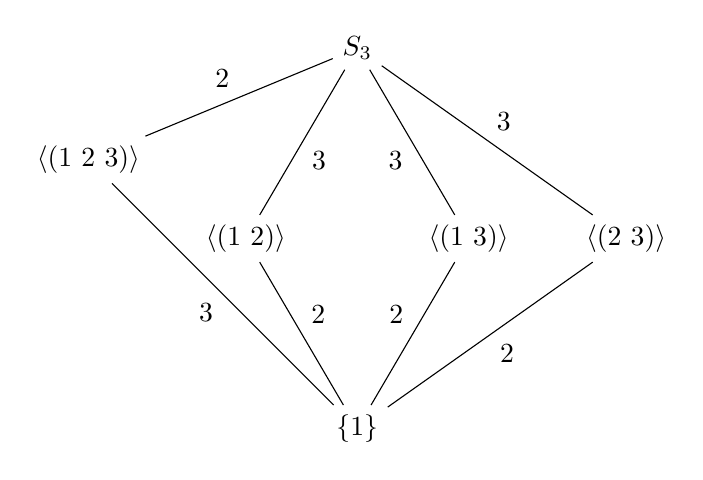
\begin{tikzpicture}[node distance=2cm]
                    \node (S3) {$S_3$};
                    \node (1) [below left of=S3, yshift=-1cm] {$\left\langle (1\ 2)\right\rangle$};
                    \node (2) [below right of=S3, yshift=-1cm] {$\left\langle (1\ 3)\right\rangle$};
                    \node (3) [left of=1, yshift=1cm] {$\left\langle (1\ 2\ 3)\right\rangle$};
                    \node (4) [right of=2] {$\left\langle (2\ 3)\right\rangle$};
                    \node (5) [below right of=1, yshift=-1cm] {$\{1\}$};
                    
                    \draw (S3) -- node[below right] {$3$} (1);
                    \draw (S3) -- node[below left] {$3$} (2);
                    \draw (S3) -- node[above left] {$2$} (3);
                    \draw (S3) -- node[above right] {$3$} (4);
                    \draw (1) -- node[above right] {$2$} (5);
                    \draw (2) -- node[above left] {$2$} (5);
                    \draw (3) -- node[below left] {$3$} (5);
                    \draw (4) -- node[below right] {$2$} (5);
                \end{tikzpicture}
                \caption{Diagrama de Hasse para los subgrupos de $S_3$.}
            \end{figure}
            Como $A_3 = \langle (1\ 2\ 3) \rangle \lhd S_3$ (por tener índice 2) y ningún otro subgrupo de $S_3$ es normal salvo el trivial, la única serie de composición de $S_3$ es:
            \begin{equation*}
                S_3 \rhd A_3 \rhd \{1\}
            \end{equation*}
        \item En $D_4$:
            \begin{figure}[H]
                \centering
                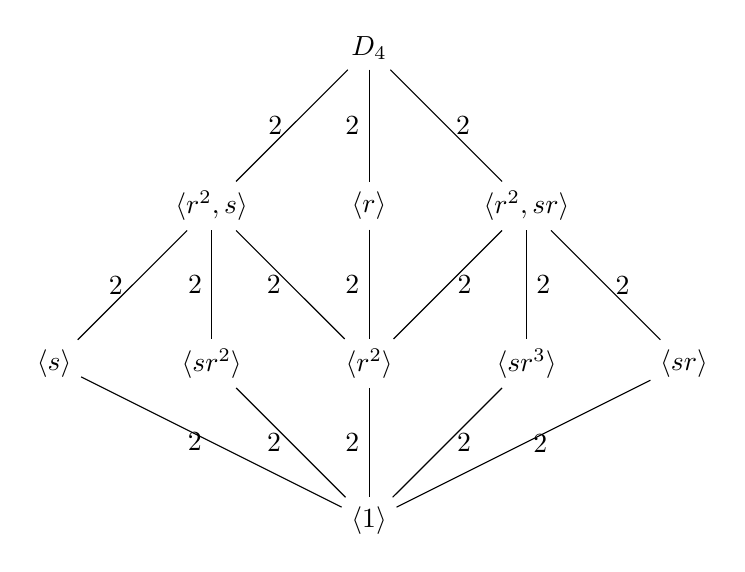
\begin{tikzpicture}[node distance=2cm]
                    \node (D4) {$D_4$};
                    \node[below of=D4] (r) {$\langle r\rangle$};
                    \node[left of=r] (r2s) {$\langle r^2,s\rangle$};
                    \node[right of=r] (r2sr) {$\langle r^2,sr\rangle$};
                    \node[below of=r] (r2) {$\langle r^2\rangle$};
                    \node[left of=r2] (sr2) {$\langle sr^2\rangle$};
                    \node[right of=r2] (sr3) {$\langle sr^3\rangle$};
                    \node[right of=sr3] (sr) {$\langle sr\rangle$};
                    \node[left of=sr2] (s) {$\langle s\rangle$};
                    \node[below of=r2] (1) {$\langle 1\rangle$};

                    \draw (D4) --node[left] {$2$} (r);
                    \draw (D4) --node[left] {$2$} (r2s);
                    \draw (D4) --node[right] {$2$} (r2sr);
                    \draw (r) --node[left] {$2$} (r2);
                    \draw (r2s) --node[left] {$2$} (sr2);
                    \draw (r2s) --node[left] {$2$} (s);
                    \draw (r2s) --node[left] {$2$} (r2);
                    \draw (r2sr) --node[right] {$2$} (sr3);
                    \draw (r2sr) --node[right] {$2$} (sr);
                    \draw (r2sr) --node[right] {$2$} (r2);
                    \draw (r2) --node[left] {$2$} (1);
                    \draw (sr2) --node[left] {$2$} (1);
                    \draw (sr3) --node[right] {$2$} (1);
                    \draw (sr) --node[right] {$2$} (1);
                    \draw (s) --node[left] {$2$} (1);
                \end{tikzpicture}
                \caption{Diagrama de Hasse para los subgrupos de $D_4$.}
            \end{figure}
            Como todos los índices del grafo son 2, todas las relaciones de inclusión mostradas en el grafo en realidad son relaciones de normalidad ($\lhd$), por lo que tenemos 7 series de composición distintas (una por cada forma que tengamos de llegar desde $D_4$ hasta $\{1\}$ en el grafo mediante caminos descendientes):
            \begin{align*}
                D_4 &\rhd \langle r^2, s \rangle \rhd  \langle s \rangle  \rhd \{1\} \\
                D_4 &\rhd \langle r^2, s \rangle \rhd \langle sr^2 \rangle  \rhd \{1\} \\
                D_4 &\rhd \langle r^2, s \rangle \rhd \langle r^2 \rangle  \rhd \{1\} \\
                D_4 &\rhd \langle r^2, sr \rangle  \rhd \langle r^2 \rangle  \rhd \{1\} \\
                D_4 &\rhd \langle r^2, sr \rangle  \rhd \langle sr \rangle  \rhd \{1\} \\
                D_4 &\rhd \langle r^2, sr \rangle  \rhd \langle sr^3 \rangle  \rhd \{1\} \\
                D_4 &\rhd \langle r \rangle \rhd \langle r^2 \rangle  \rhd \{1\}
            \end{align*}
        \item Para $A_4$:

            \begin{figure}[H]
                \centering
                \shorthandoff{""}
\begin{tikzcd}
                                                      &                                                     & A_4 \arrow[rrd, "3", no head] \arrow[rdd, "4", no head] \arrow[dd, "4", no head] \arrow[ldd, "4", no head] \arrow[lldd, "4"', no head] &                                                        &                                                                                &                                                         \\
                                                      &                                                     &                                                                                                                                        &                                                        & V \arrow[ldd, "2", no head] \arrow[dd, "2", no head] \arrow[rdd, "2", no head] &                                                         \\
\langle (1\ 2\ 3) \rangle \arrow[rrdd, "3"', no head] & \langle (1\ 2\ 4) \rangle \arrow[rdd, "3", no head] & \langle (1\ 3\ 4) \rangle \arrow[dd, "3", no head]                                                                                     & \langle (2\ 3\ 4) \rangle \arrow[ldd, "3"', no head]   &                                                                                &                                                         \\
                                                      &                                                     &                                                                                                                                        & \langle (1\ 3)(2\ 4) \rangle \arrow[ld, "2"', no head] & \langle (1\ 3)(2\ 4) \rangle \arrow[lld, "2"', no head]                        & \langle (1\ 4)(2\ 3) \rangle \arrow[llld, "2", no head] \\
                                                      &                                                     & \{1\}                                                                                                                                  &                                                        &                                                                                &                                                        
\end{tikzcd}
                \shorthandon{""}
            \end{figure}
            Como $V\lhd A_4$, tenemos como series de composición:
            \begin{align*}
                A_4 &\rhd V \rhd \langle (1\ 2)(3\ 4) \rangle  \rhd \{1\} \\
                A_4 &\rhd V \rhd \langle (1\ 3)(2\ 4) \rangle  \rhd \{1\} \\
                A_4 &\rhd V \rhd \langle (2\ 3)(2\ 3) \rangle  \rhd \{1\} 
            \end{align*}
            Además, como ninguna de las relaciones $\langle (i\ j\ k) \rangle < A_4 $ es normal, no tenemos más series de composición.
        \item En $D_5 = \langle r,s\mid r^5 = s^2 = 1, sr = r^4 s \rangle $ tenemos:

            \begin{figure}[H]
                \centering
                \shorthandoff{""}
\begin{tikzcd}
                                             &  & D_5 \arrow[lld, "2", no head] \arrow[dd, "5"', no head] \arrow[rdd, "5"', no head] \arrow[rrdd, "5"', no head] \arrow[rrrdd, "5"', no head] \arrow[rrrrdd, "5", no head] &                                              &                                                 &                                                  &                                                  \\
\langle r \rangle \arrow[rrdd, "5", no head] &  &                                                                                                                                                                          &                                              &                                                 &                                                  &                                                  \\
                                             &  & \langle s \rangle \arrow[d, "2"', no head]                                                                                                                               & \langle sr \rangle \arrow[ld, "2"', no head] & \langle sr^2 \rangle \arrow[lld, "2"', no head] & \langle sr^3 \rangle \arrow[llld, "2"', no head] & \langle sr^4 \rangle \arrow[lllld, "2", no head] \\
                                             &  & \{1\}                                                                                                                                                                    &                                              &                                                 &                                                  &                                                 
\end{tikzcd}
                \shorthandon{""}
            \end{figure}
            Solo tenemos la serie de composición:
            \begin{equation*}
                D_5 \rhd \langle r \rangle  \rhd \{1\}
            \end{equation*}
            Ya que $D_5$ no tiene más subgrupos normales, a parte del trivial.
        \item En el grupo de los cuaternios:
            \begin{figure}[H]
                \centering
                \begin{tikzpicture}[node distance=2cm]
                    \node (Q2) {$Q_2$};
                    \node (1) [below of=Q2, xshift=-2cm] {$\left\langle i\right\rangle$};
                    \node (2) [below of=Q2] {$\left\langle j\right\rangle$};
                    \node (3) [below of=Q2, xshift=2cm] {$\left\langle k\right\rangle$};
                    \node (4) [below of=2] {$\left\langle -1\right\rangle$};
                    \node (5) [below of=4] {$\{1\}$};

                    \draw (Q2) -- node[above left] {$2$} (1);
                    \draw (Q2) -- node[left] {$2$} (2);
                    \draw (Q2) -- node[above right] {$2$} (3);
                    \draw (1) -- node[below left] {$2$} (4);
                    \draw (2) -- node[left] {$2$} (4);
                    \draw (3) -- node[below right] {$2$} (4);
                    \draw (4) -- node[left] {$2$} (5);
                \end{tikzpicture}
                \caption{Diagrama de Hasse para los subgrupos del grupo de los cuaternios.}
            \end{figure}
            Como todas las aristas del grafo están numeradas con índice 2, todas las relaciones de subgrupo son normales, por lo que tenemos 3 series de composición, una por cada camino posible:
            \begin{align*}
                Q_2 &\rhd \langle i \rangle  \rhd \langle -1 \rangle  \rhd \{1\} \\
                Q_2 &\rhd \langle j \rangle  \rhd \langle -1 \rangle  \rhd \{1\} \\
                Q_2 &\rhd \langle k \rangle  \rhd \langle -1 \rangle  \rhd \{1\} 
            \end{align*}
        \item En $S_3\times \mathbb{Z}_2$:
            Por una parte, en $S_3$ teníamos una única serie de composición:
            \begin{equation*}
                S_3 \rhd A_3 \rhd \{1\}
            \end{equation*}
            Y en $\mathbb{Z}_2$ la única opción a considerar es $\mathbb{Z}_2 \rhd \{0\}$.
            Podemos considerar ahora las series de composición resultantes de considerar todas las combinaciones:
            \begin{align*}
                S_3\times \mathbb{Z}_2 &\rhd S_3 \times \{0\} \rhd A_3\times \{0\} \rhd \{(1,0)\} \\
                S_3\times \mathbb{Z}_2 &\rhd A_3\times \mathbb{Z}_2 \rhd A_3 \times \{0\} \rhd \{(1,0)\} \\
                S_3\times \mathbb{Z}_2 &\rhd A_3\times \mathbb{Z}_2 \rhd \{1\}\times \mathbb{Z}_2 \rhd \{(1,0)\}
            \end{align*}
            Que obtenemos primero variando algunos y luego otras. Esto es posible ya que el producto de subgrupos es subgrupo del producto, como vimos en la Proposición~\ref{prop:monomorfismo_aut}.

            Sin embargo, como $\mcd(6,2) = 2 \neq 1$, el Teorema~\ref{teo:grupos_finitos_producto} no puede asegurarnos que todos los subgrupos de $S_3\times \mathbb{Z}_2$ sean producto de subgrupos, y de hecho vamos a tener que hay subgrupos del producto que no son producto de subgrupos de cada coordenada, por lo que tendremos otra serie de composición, que tendrá la forma:
            \begin{equation*}
                S_3\times \mathbb{Z}_2 \stackrel{2}{\rhd} H_1 \stackrel{2}{\rhd} H_2 \stackrel{3}{\rhd} \{1\}
            \end{equation*}
            Con $H_1,H_2 < S_3\times \mathbb{Z}_2$ que no especificaremos pero diremos que $H_1\cong S_3$ y $H_2\cong A_3$.
    \end{itemize}
\end{ejemplo}

\begin{definicion}[Grupo simple]
    Un grupo $G$ se dice simple si no es trivial y no tiene subgrupos normales propios
\end{definicion}

\begin{ejemplo}
    $\mathbb{Z}_3$ es un grupo simple, ya que su retículo de subgrupos es:
    \begin{figure}[H]
        \centering
        \shorthandoff{""}
        \begin{tikzcd}
        \mathbb{Z}_3 \arrow[d, no head] \\
        \{0\}                          
        \end{tikzcd}
        \shorthandon{""}
    \end{figure}
    \noindent
    Un resultado que veremos luego (el Teorema de Abel) nos dirá que los grupos $A_n$ para $n\geq 5$ son grupos simples.
\end{ejemplo}

\subsubsection{Resultados sobre series de composición}
\begin{prop}\label{prop:carac_simples_abelianos}
    Un grupo abeliano finito es simple si y solo si es un grupo cíclico de orden primo.
    \begin{proof}
        Por doble implicación:
        \begin{description}
            \item [$\Longleftarrow)$] Si $G$ es cíclico de orden primo, no va a tener subgrupos propios, por lo que será simple.
            \item [$\Longrightarrow)$] Si $G$ es abeliano, entonces todos sus subgrupos serán normales. Si es simple, no tendrá subgrupos propios (ya que si no serían normales, luego no sería simple). Sea $1\neq x\in G$, sabemos que $\langle x \rangle < G$, de donde ($\{1\}\neq \langle x \rangle $ y $G$ no tiene subgrupos propios) $G = \langle x \rangle $, por lo que $G$ es cíclico. 

                Si $|G| = nm$, entonces $\{1\}\neq \langle x^m \rangle < G$, por lo que $G$ tendría subgrupos propios, luego no sería simple. Por tanto, $|G|$ ha de ser primo.
        \end{description}
    \end{proof}
\end{prop}

\begin{ejemplo}
    Estudiando un poco el caso de grupos cíclicos infinitos, $\mathbb{Z}$ no es simple, ya que tiene subgrupos propios (que además son normales, por ser $\mathbb{Z}$ abeliano).
\end{ejemplo}

\begin{prop}[Caracterización de series de composición]
    Sea $G$ un grupo, una serie normal es de composición si y solo si sus factores son grupos simples.
    \begin{proof}
        Consideramos una serie normal de longitud $r$:
        \begin{equation*}
            G = G_0 \rhd G_1 \rhd \ldots \rhd G_r = \{1\}
        \end{equation*}
        Y demostraremos que la serie no es de composición si y solo si tiene un factor que no es un grupo simple:
        \begin{description}
            \item [$\Longrightarrow)$] Si la serie no es de composición, podemos encontrar $H<G$ de forma que la serie:
                \begin{equation*}
                    G = G_0 \rhd \ldots \rhd G_{k-1} \rhd H \rhd G_k \rhd \ldots \rhd G_r = \{1\}
                \end{equation*}
                Sea un refinamiento normal propio de la serie de partida. Si consideramos la proyección al cociente de los grupos:
                \begin{equation*}
                    G_{k-1} \rhd H \rhd G_k
                \end{equation*}
                Llegamos a que:
                \begin{equation*}
                    p_\ast(G_{k-1}) = G_{k-1}/G_k \rhd p_\ast(H) = H/G_k \rhd p_\ast(G_k) = \{G_k\}
                \end{equation*}
                Y ninguna de estas inclusiones es una igualdad, ya que:
                \begin{itemize}
                    \item Si $G_{k-1}/G_k = H/G_k$, entonces $G_{k-1} = H$ y el refinamiento anterior no era propio.
                    \item Si $H/G_k = \{G_k\}$, entonces $H = G_k$ y el refinamiento anterior no era propio.
                \end{itemize}
                En definitiva, hemos encontrado un subgrupo normal propio de $G_{k-1}/G_k$, por lo que este factor no es un grupo simple.
            \item [$\Longleftarrow)$] Si existe $k\in \{1,\ldots,r\}$ de forma que $G_{k-1}/G_k$ no es un grupo simple, entonces dicho grupo tendrá un subgrupo propio normal suyo:
                \begin{equation*}
                    \{G_k\} = \{1\} \neq H \lhd G_{k-1}/G_k
                \end{equation*}
                Si usamos el Tercer Teorema de Isomorfía considerando la proyección al cociente $p_k:G_{k-1}\to G_{k-1}/G_k$, tenemos que:
                \begin{equation*}
                    p^\ast_k(H) \lhd G_{k-1}
                \end{equation*}
                Además, como $H < G_{k-1}/G_k$, tendremos que $G_k \in H$, luego:
                \begin{equation*}
                    G_k = \ker(p_k) = p_k^\ast(\{G_k\}) \subseteq p_k^\ast(H) \lhd G_{k-1}
                \end{equation*}
                Y por ser $G_k \lhd G_{k-1}$, deducimos que también $G_k\lhd p_k^\ast(H)$. Hemos encontrado un subgrupo normal de $G$ que estaría entre $G_k$ y $G_{k-1}$:
                \begin{equation*}
                    G = G_0 \rhd \ldots \rhd G_{k-1} \rhd p_k^\ast(H) \rhd G_k \rhd \ldots \rhd G_r = \{1\}
                \end{equation*}
                Además, este refinamiento de la serie normal es propio, ya que:
                \begin{itemize}
                    \item Si fuese $p_k^\ast(H) = G_k$, tendríamos que $H = \{G_k\}$.
                    \item Si fuese $p_k^\ast(H) = G_{k-1}$, tendríamos que $H = G_{k-1}/G_k$.
                \end{itemize}
                Ambos casos son imposibles, puesto que $H$ era un subgrupo propio de $G_{k-1}/G_k$. Hemos encontrado un refinamiento normal propio de la serie de partida, por lo que esta no era de composición.
        \end{description}
    \end{proof}
\end{prop}

\begin{prop}
    Todo grupo finito tiene una serie de composición.
    \begin{proof}
        Sea $G$ un grupo finito, distinguimos casos:
        \begin{itemize}
            \item Si $G$ es simple o trivial, entonces no tiene subgrupos normales propios, por lo que tiene una única serie de composición:
                \begin{equation*}
                    G \rhd \{1\}
                \end{equation*}
            \item Si $|G| = p$ primo, vimos en la Proposición~\ref{prop:grupo_primo} que entonces $G$ es cíclico, y la Proposición~\ref{prop:carac_simples_abelianos} nos dice que $G$ es simple, por lo que estamos en el caso anterior.
            \item Si $|G|$ no es primo y $G$ no es simple, por inducción sobre $n = |G|$, suponemos que es cierto para todo grupo $H$ con $|H|<|G|$ (observemos que el punto anterior nos sirve como caso base).

                Como $G$ es finito, tiene un número finito de subgrupos, entre los que podemos encontrar (por ser $G$ no simple) $G_1$, un subgrupo normal propio maximal\footnote{Es decir, que no existe $G_1 \neq K\lhd G$ con $G_1 \lhd  K$.} de $G$. Como $|G_1| < |G|$ ($G_1$ es subgrupo propio), por hipótesis de inducción tenemos una serie de composición para $G_1$:
                \begin{equation*}
                    G_1 \rhd G_2 \rhd \ldots \rhd G_r = \{1\}
                \end{equation*}
                Además, como $G_1$ era el subgrupo normal maximal de $G$, sabemos que no existe $H\lhd G$ con $G_1 \lhd H \lhd G$, por lo que la serie:
                \begin{equation*}
                    G = G_0 \rhd G_1 \rhd G_2 \rhd \ldots \rhd G_r = \{1\}
                \end{equation*}
                Es de composición. \qedhere
        \end{itemize}
    \end{proof}
\end{prop}

\begin{teo}[de Refinamiento de Schreier]
    Sea $G$ un grupo, dos series normales de $G$ tienen refinamientos isomorfos.
    \begin{proof}
        Consideramos dos series normales de $G$:
        \begin{equation}\label{eq:teo_1}
            G = G_0 \rhd G_1 \rhd \ldots \rhd G_{i-1} \rhd G_i \rhd \ldots\rhd G_r = \{1\} \\
        \end{equation}
        \begin{equation}\label{eq:teo_2}
            G = H_0 \rhd H_1 \rhd \ldots \rhd H_{j-1} \rhd H_j \rhd \ldots \rhd H_s = \{1\}
        \end{equation}
        Fijado $i \in \{1,\ldots,r\}$, tenemos $G_i \lhd G_{i-1} < G$, y para todo $j \in \{1,\ldots,s\}$ tenemos $H_j\lhd H_{j-1} < G$, donde podemos aplicar el primer apartado del Cuarto Teorema de Isomorfía, obteniendo la siguiente relación entre los grupos:
        \begin{equation*}
            G_{ij} = G_i(H_j\cap G_{i-1}) \lhd G_i(H_{j-1}\cap G_{i-1}) = G_{ij-1} \qquad \forall j\in \{1, \ldots, s\}
        \end{equation*}
        En los casos extremos (es decir, en $j = 0$ y $j = s$), tendremos:
        \begin{align*}
            G_{i0} &= G_i(H_0\cap G_{i-1}) = G_iG_{i-1} = G_{i-1} \\
            G_{is} &= G_i(H_s\cap G_{i-1}) = G_i \{1\} = G_i
        \end{align*}
        De esta forma, tenemos para todo $i \in \{1,\ldots,r\}$ que:
        \begin{equation*}
            G_{i-1} = G_{i0} \rhd G_{i1} \rhd \ldots \rhd G_{is-1} \rhd G_{is} = G_i
        \end{equation*}
        Que podemos meter en todos los eslabones de la serie~(\ref{eq:teo_1}):
        \begin{multline*}
            G = G_0 = G_{10} \rhd G_{11} \rhd \ldots \rhd G_{1s} = G_1 = G_{20} \rhd G_{21} \rhd \ldots \rhd G_{2s} = G_2 = G_{30} \rhd \ldots  \\
            \ldots \rhd G_{r-1s} = G_{r-1} = G_{r0} \rhd \ldots \rhd G_{rs} = G_r =  \{1\}
        \end{multline*}
        Obteniendo un refinamiento de longitud $r(s+1)-(r-1) = rs + 1$:\newline
        En cada eslabón (teníamos $r$) hemos metido $s+1$ eslabones, de los que se repetían ($G_{is} = G_{i+1,0}$, para $i \in \{0, \ldots, r-1\}$) $r-1$ eslabones.\\

        \noindent
        Si repetimos el procedimiento para la serie~(\ref{eq:teo_2}), fijado $j\in \{1,\ldots,s\}$, para todo $i \in \{0,\ldots, r\}$ podemos aplicar el primer apartado del Cuarto Teorema de Isomorfía, obteniendo que:
        \begin{equation*}
            H_{ij} = H_j(G_i\cap H_{j-1}) \lhd H_j(G_{i-1}\cap H_{j-1}) = H_{i-1j} \qquad \forall i \in \{1, \ldots, r\}
        \end{equation*}
        En los casos extremos tendremos:
        \begin{align*}
            H_{0j} &= H_{j-1} \\
            H_{rj} &= H_j
        \end{align*}
        Por lo que para todo $j \in \{1, \ldots, s\}$, tenemos:
        \begin{equation*}
            H_{j-1} = H_{0j} \rhd H_{1j} \rhd \ldots \rhd H_{r-1j} \rhd H_{rj} = H_j
        \end{equation*}
        Y podemos obtener un refinamiento de~(\ref{eq:teo_2}) al igual que hicimos antes, metiendo la cadena superior entre cada uno de los eslabones de la serie original:
        \begin{multline*}
            G = H_0 = H_{01} \rhd H_{11} \rhd \ldots \rhd H_{r1} = H_1 = H_{02} \rhd H_{12} \rhd \ldots \rhd H_{r2} = G_2 = H_{03} \rhd \ldots \\
            \ldots \rhd H_{rs-1} = H_{s-1} = H_{0s} \rhd H_{1s} \rhd \ldots \rhd H_{rs} = H_s = \{1\}
        \end{multline*}
        Que tiene longitud $s(r+1)-(s-1) = rs+1$, al igual que antes.\\

        \noindent
        Ahora, por la segunda parte del Cuarto Teorema de Isomorfía, tenemos que:
        \begin{equation*}
            \dfrac{G_{ij-1}}{G_{ij}} = \dfrac{G_i(H_j\cap G_{i-1})}{G_i(H_j\cap G_{i-1})} \cong \dfrac{H_j(G_{i-1}\cap H_{j-1})}{H_j(G_i \cap H_{j-1})} = \dfrac{H_{i-1j}}{H_{ij}}
        \end{equation*}
        Por lo que los dos refinamientos encontrados son isomorfos.
    \end{proof}
\end{teo}

\begin{ejercicio*}
    Se pide calcular un refinamiento isomorfo aplicando el método de Schreier a las dos siguientes series normales:
    \begin{align*}
        G &= G_0 \rhd G_1 \rhd G_2 \rhd G_3 = \{1\} \\
        G &= H_0 \rhd H_1 \rhd H_2 = \{1\}
    \end{align*}
\end{ejercicio*}

\begin{teo}[Jordan-Holder]
    Si un grupo $G$ admite una serie de composición, cualquier serie normal puede refinarse a una serie de composición.\\

    \noindent
    Además, dos series de composición de un mismo grupo son isomorfas siempre.
    \begin{proof}
        Tomamos una serie de composición de $G$:
        \begin{equation*}
            G= G_0 \rhd G_1 \rhd \ldots \rhd G_r = \{1\}
        \end{equation*}
        Y también una serie normal de $G$:
        \begin{equation*}
            G=H_0 \rhd H_1 \rhd \ldots \rhd H_s = \{1\}
        \end{equation*}
        Por el Teorema de Schreier (la serie de composición es normal), existe un refinamiento de ambos isomorfo. Sin embargo, como la primera serie es de composición, su refinamiento coincide con ella misma. Para la segunda serie, obtendremos un refinamiento isomorfo a la primera:
        \begin{equation*}
            G = \overline{G_0} \rhd \overline{G_1} \rhd \ldots \rhd \overline{G_r} = \{1\}
        \end{equation*}
        Por tanto, tendremos que $\exists \sigma\in S_r$ de forma que:
        \begin{equation*}
            G_k/G_{k+1} \cong \overline{G}_{\sigma(k)}/\overline{G}_{\sigma(k)+1} \qquad \forall k \in \{0,\ldots,r-1\}
        \end{equation*}
        Como la primera serie era de composición, los factores $G_k/G_{k+1}$ son simples, y como esta propiedad se conserva por isomorfismos (compruébese), los factores $\overline{G}_k/\overline{G}_{k+1}$ también serán simples, de donde deducimos que el refinamiento de la serie normal que hemos encontrado es de composición.
    \end{proof}
\end{teo}

\noindent
Con este último Teorema de Jordan-Holder se tiene claro ya el interés en las series de composición, ya que cada grupo admite un única (salvo isomorfismos) serie de composición.\\

\noindent
Podemos pensar en calcular series de composición de un grupo conocida una serie de composición en un grupo isomorfo, resultado que podemos esperar que sea cierto (y que de hecho vamos a probar a continuación); sin embargo, el recíproco no es cierto en general: si tenemos dos series de composición isomorfas, una de un grupo $G$ y otra de otro grupo $K$, en general $G$ y $K$ no van a ser isomorfos.

\begin{ejemplo}
    Por ejemplo, anteriormente vimos en un ejemplo que la única serie de composición que podemos considerar en $S_3$ es:
    \begin{equation*}
        S_3 \stackrel{2}{\rhd} A_3 \stackrel{3}{\rhd} \{1\}
    \end{equation*}
    En $\mathbb{Z}_6$, que no es isomorfo a $S_3$ por ser abeliano, si observamos su retículo:
            \begin{figure}[H]
                \centering
                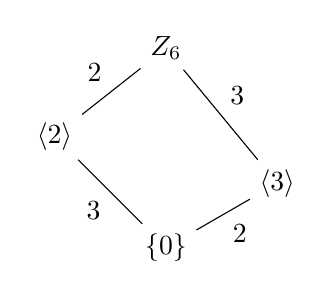
\begin{tikzpicture}[node distance=2cm]
                    \node (Z6) {$\bb{Z}_6$};
                    \node (2) [below left of=Z6, yshift=.3cm] {$\langle 2 \rangle$};
                    \node (3) [below right of=Z6, yshift=-.3cm] {$\langle 3 \rangle$};
                    \node (0) [below right of=2] {$\{0\}$};

                    \draw (Z6) -- node[above left] {$2$} (2);
                    \draw (Z6) -- node[above right] {$3$} (3);
                    \draw (2) -- node[below left] {$3$} (0);
                    \draw (3) -- node[below right] {$2$} (0);
                \end{tikzpicture}
                \caption{Diagrama de Hasse para los subgrupos de $\mathbb{Z}_6$.}
            \end{figure}
            Vemos que una serie de composición de $\mathbb{Z}_6$ es:
            \begin{equation*}
                \mathbb{Z}_6 \stackrel{2}{\rhd} \langle 2 \rangle  \stackrel{3}{\rhd} \{0\}
            \end{equation*}
            Además, sabemos ahora por el Teorema de Jordan-Holder que $\mathbb{Z}_6$ no tiene más series de composición, ya que la otra posibilidad sería la serie:
            \begin{equation*}
                \mathbb{Z}_6 > \langle 3 \rangle > \{0\}
            \end{equation*}
            Pero como esta no es isomorfa a la primera y sabemos que todas las series de composición de un mismo grupo son isomorfas, sabemos que esta segunda no es de composición. Vemos finalmente que las series:
            \begin{gather*}
                S_3 \stackrel{2}{\rhd} A_3 \stackrel{3}{\rhd} \{1\} \\
                \mathbb{Z}_6 \stackrel{2}{\rhd} \langle 2 \rangle  \stackrel{3}{\rhd} \{0\} 
            \end{gather*}
            son isomorfas. Para ello, basta ver que:
            \begin{gather*}
                S_3/A_3 \cong \mathbb{Z}_2 \cong Z_6/\langle 2 \rangle  \\
                A_3/\{1\} \cong A_3 \cong \mathbb{Z}_3 \cong \langle 2 \rangle  \cong \langle 2 \rangle /\{0\}
            \end{gather*}
\end{ejemplo}

\noindent
Veamos ahora que dos grupos isomorfos siempre tienen una serie de composición isomorfa. Sin embargo, antes de ello, hemos de destacar un resultado que no vimos en el Capítulo anterior pero que puede demostrarse fácilmente con las herramientas introducidas en el mismo.

\begin{lema}
    Sean $G$ y $K$ dos grupos, $f:G\to K$ un isomorfismo de grupos y $H\lhd G$, entonces:
    \begin{equation*}
        G/H \cong K/f_\ast(H)
    \end{equation*}
    \begin{proof}
        En primer lugar, hemos de demostrar que $f_\ast(H)\lhd K$. Para ello:
        \begin{itemize}
            \item Como $H<G$ y $f$ es un homomorfismo, por la Proposición~\ref{prop:imagen_directa}, tenemos que $f_\ast(H) < K$.
            \item Ahora, si $y\in K$ y $h'\in f(H)$, existirán $x\in G$ y $h\in H$ de forma que:
                \begin{equation*}
                    f(x) = y \qquad f(h) = h'
                \end{equation*}
                En cuyo caso:
                \begin{equation*}
                    yh'y = f(x)f(h){(f(x))}^{-1} = f(xhx^{-1}) \in f(H)
                \end{equation*}
                Ya que por ser $H\lhd G$, tenemos que $xhx^{-1}\in H$.
        \end{itemize}
        Ahora, podemos considerar los grupos cocientes $G/H$ y $K/f_\ast(H)$, junto con las proyecciones $p_G:G\to G/H$ y $p_K:K\to K/f_\ast(H)$. Si definimos $g:G\to K/f_\ast(H)$ como $g = p_K\circ f$:
        \begin{equation*}
            g(x) = p_K(f(x)) = f(x)f_\ast(H) \qquad \forall x\in G
        \end{equation*}
        Es un homomorfismo, como composición de homomorfismos. Si observamos el siguiente diagrama:
        \begin{figure}[H]
            \centering
            \shorthandoff{""}
            \begin{tikzcd}
            G \arrow[d, "f"'] \arrow[r, "p_G"] \arrow[rd, "g"'] & G/H \arrow[d, "\varphi", dashed] \\
            K \arrow[r, "p_K"]                                  & K/f_\ast(H)                     
            \end{tikzcd}
            \shorthandon{""}
            \caption{Situación de los grupos.}
        \end{figure}
        \noindent
        Podemos aplicar la Propiedad Universal del grupo cociente sobre $g$, obteniendo que existe un único homomorfismo $\varphi:G/H\to K/f_\ast(H)$ que hace que el diagrama conmute. Como vimos en el Teorema~\ref{teo:prop_universal}:
        \begin{itemize}
            \item Como $g$ es sobreyectiva por ser composición de aplicaciones sobreyectivas, tenemos que $\varphi$ es sobreyectiva.
            \item Calculemos $\ker(g)$, sea $x\in \ker(g)$:
                \begin{equation*}
                    f(x)f_\ast(H) = p_K(f(x)) = g(x) = f_\ast(H)
                \end{equation*}
                Entonces, $f(x) \in f_\ast(H)$, de donde $x\in H$. La inclusión $H\subseteq \ker(g)$ es clara, por lo que $H = \ker(g)$, de donde deducimos que $\varphi$ es inyectiva.
        \end{itemize}
    \end{proof}
\end{lema}

\begin{prop}
    Sean $G$ y $K$ dos grupos isomorfos, entonces todas las series de composición de $G$ son isomorfas a todas las series de composición de $K$.
    \begin{proof}
        Como todas las series de composición de $G$ son isomorfas entre sí y todas las series de composición de $K$ también (por el Teorema de Jordan-Holder), basta ver que hay una serie de composición de $G$ que es isomorfa a una serie de composición de $K$. Para ello, como $G\cong K$, ha de existir un isomorfismo de grupos $f:G\to K$. Sea
        \begin{equation*}
            G = G_0 \rhd G_1 \rhd \ldots \rhd G_r = \{1\} 
        \end{equation*}
        una serie de composición de $G$, si denotamos:
        \begin{equation*}
            H_k = f_\ast(G_k) \qquad \forall k\in \{0,\ldots,r\}
        \end{equation*}
        Tendremos entonces una serie normal en $K$:
        \begin{equation*}
            K = H_0 \rhd H_1 \rhd \ldots \rhd H_r = \{1\}
        \end{equation*}
        Por el Lema anterior, tenemos que:
        \begin{equation*}
            G_k/G_{k+1} \cong H_k/H_{k+1} \qquad \forall k\in \{0,\ldots,r-1\}
        \end{equation*}
        Además, como la serie de $G$ era de composición, sus factores serán grupos simples, de donde los factores $H_k/H_{k+1}$ serán también grupos simples, por lo que la serie obtenida en $K$ es de composición, y son series isomorfas.
    \end{proof}
\end{prop}~\\

\noindent
El objetivo principal de esta asignatura es clasificar los grupos finitos. Como estos grupos van a tener series de composición cuyos factores serán grupos simples, nos centraremos en clasificar los grupos simples, para luego clasificar los grupos finitos.\\

\noindent
La teoría de clasificación de grupos simples comenzó en 1960 y fue completada en 2004, con una demostración de 15000 páginas en lo que se conoce como el ``Teorema enorme''. En la demostración intervinieron matemáticos como Gorestein (1923 - 1992). Esta clasificación de los grupos simples se hizo en:
\begin{itemize}
    \item 18 familias infinitas de grupos simples.
    \item 26 grupos simples, llamados grupos esporádicos. 

        Como curiosidad, el grupo esporádico más pequeño tiene orden 7920 y el más grande, $10^{54}$.
\end{itemize}
Cualquier grupo finito simple pertenece a una de estas 18 familias, o es isomorfo a alguno de los 26 grupos esporádicos.\\

\noindent
Entre las 18 familias de grupos simples destacamos 2, que son las que nos interesan por ahora: 
\begin{itemize}
    \item Los grupos cíclicos de orden primo, que ya hemos demostrado que se tratan de grupos simples.
    \item Los grupos alternados $A_n$ con $n\geq 5$.
\end{itemize}
Veremos ahora este segundo resultado, en el ya prometido Teorema de Abel.

\begin{teo}[de Abel]
    $A_n$ es simple, para $n\geq 5$.
    \begin{proof} 
        Sea $\{1\} \neq N \lhd A_n$, veamos que ha de ser $N = A_n$. En la Proposición~\ref{prop:generadores_grupos} vimos que dado\footnote{Donde $X_n = \{1,2,\ldots,n\}.$} $j \in X_n\setminus \{1,2\}$, teníamos que:
        \begin{equation*}
            A_n = \langle (1\ 2\ j) \rangle 
        \end{equation*}
        Y la demostración terminará viendo que $N$ contiene a un elemento de esta forma. Bajo estas hipótesis, sabemos que va a existir (por ser $N$ finito) $1\neq \sigma\in N$, la permutación de $N$ que mueve menos elementos. Por ser $\sigma$ par (estamos en $A_n$), ha de mover más de dos elementos. Veamos que mueve exactamente 3:
        \begin{enumerate}
            \item Si $\sigma$ es producto de ciclos disjuntos de longitud 2: supongamos que $\sigma$ mueve, al menos, los elementos $x_1,x_2,x_3$ (distintos entre sí), con lo que podemos escribir:
                \begin{equation*}
                    \sigma = (x_1\ x_2)(x_3\ x_4) \ldots
                \end{equation*}
                Sea $\tau = (x_3\ x_4\ x_5)$ para ciertos $x_4,x_5\in X_n$ distintos de $x_1,x_2,x_3$ y distintos entre sí, definimos:
                \begin{equation*}
                    \sigma_1 = (x_3\ x_4\ x_5)\sigma {(x_3\ x_4\ x_5)}^{-1}\in  N
                \end{equation*}
                $\sigma_1$ está en $N$ por ser $N\lhd A_n$. Si consideramos:
                \begin{equation*}
                    [\tau, \sigma] = \tau \sigma \tau^{-1} \sigma^{-1} = \sigma_1 \sigma^{-1} \in N
                \end{equation*}
                \begin{itemize}
                    \item Supongamos que $\sigma$ mueve a $x_5$, en cuyo caso:
                        \begin{gather*}
                            \sigma = (x_1\ x_2)(x_3\ x_4)(x_5\ \sigma(x_5))\ldots \\
                            \sigma_1 = (x_1\ x_2)(x_3\ \sigma(x_5))(x_4\ x_5)\ldots
                        \end{gather*}
                        Con lo que:
                        \begin{equation*}
                            [\tau, \sigma] = (x_3\ \sigma(x_5))(x_4\ x_5)(x_3\ x_4)(x_5\ \sigma(x_5))
                        \end{equation*}
                        Luego $[\tau, \sigma]$ deja fijos a $x_1$ y $x_2$ y mueve a los mismos que movía $\sigma$. Por ello, $[\tau, \sigma]\in N$ y $[\tau, \sigma]$ mueve menos elementos que $\sigma$, contradicción, que viene de suponer que $\sigma$ mueve a $x_5$.
                    \item Si suponemos que $\sigma$ no mueve a $x_5$:
                        \begin{equation*}
                            \sigma_1 = (x_1\ x_2)(x_4\ x_5)
                        \end{equation*}
                        Tenemos:
                        \begin{equation*}
                            [\tau, \sigma] = (x_3\ x_5\ x_4)
                        \end{equation*}
                        Que mueve menos elementos que $\sigma$, contradicción.
                \end{itemize}
                Por tanto, $\sigma$ no puede ser producto de transposiciones, ya que llegamos a contradicciones.
            \item Si $\sigma$ tiene un ciclo de longitud mayor o igual que 3 en el que mueve a $x_1,x_2$ y $x_3$, si definimos:
                \begin{align*}
                    \tau &= (x_3\ x_4\ x_5) \\
                    \sigma_1 &= \tau \sigma \tau^{-1}  \in N
                \end{align*}
                Supongamos que $\sigma$ mueve más de 3 elementos, por lo que mueve al menos (por ser una permutación par) 5. En dicho caso:
                \begin{equation*}
                    \sigma_1 = (x_1\ x_2\ x_4\ \ldots) \neq \sigma
                \end{equation*}
                Por lo que:
                \begin{equation*}
                    [\tau, \sigma] = \sigma_1 \sigma^{-1} \in N
                \end{equation*}
                Y $[\tau, \sigma]$ deja fijos a los mismos que $\sigma$ y a $x_2$. En dicho caso, tenemos que $[\tau, \sigma]$ mueve menos que $\sigma$.
        \end{enumerate}
        En definitiva, concluimos que $\sigma$ contiene a un ciclo de longitud 3, a saber: $(i\ j\ k)$, todos ellos elementos distintos.

        \begin{itemize}
            \item Si $i,j,k,1,2$ son todos distintos:
                \begin{equation*}
                    (1\ i)(2\ j)(i\ j\ k)(1\ i)(2\ j) = (1\ 2\ k) \in N
                \end{equation*}
            \item Si $i = 1$ y $j, k, 2$ fueran distintos, $\exists h$ distinto de los anteriores de forma que:
                \begin{equation*}
                    (2\ j)(k\ h)(1\ j\ k)(2\ j)(k\ h) = (1\ 2\ h) \in N
                \end{equation*}
            \item Si $i = 2$ y $j, k, 1$ fueran distintos, $\exists h$ distinto de los anteriores de forma que:
                \begin{equation*} 
                    (1\ j)(k\ h)(j\ 2\ k)(1\ j)(k\ h) = (1\ 2\ h) \in N
                \end{equation*}
        \end{itemize}
        En definitiva, $N$ contiene al generador de $A_n$, de donde:
        \begin{equation*}
            A_n = \langle (1\ 2\ j) \rangle  \subseteq N
        \end{equation*}
    \end{proof}
\end{teo}

\section{Grupos resolubles}
Antes de pasar con la definición de grupos resolubles, hemos de repasar ciertos conceptos relacionados con la operación de conmutador que ya definimos sobre los elementos de $G$, recordamos que era la aplicación $[\cdot ,\cdot ]:G\times G\to G$ dada por:
\begin{equation*}
    [x,y] = xy{(yx)}^{-1} = xyx^{-1}y^{-1} \qquad \forall x,y\in G
\end{equation*}

\subsection{Preliminares}
\noindent
Sobre el conmutador solo vimos la Proposición~\ref{prop:primer_conmutador}, que nos decía que dados dos elementos $h,k$ de un grupo $G$:
\begin{equation*}
    hk = kh \Longleftrightarrow [h,k] = 1
\end{equation*}

\begin{prop}\label{prop:props_conmutador}
    Sea $G$ un grupo y $x,y\in G$, se verifican:
    \begin{itemize}
        \item[$i)$] ${[x,y]}^{-1} = [y,x]$.
        \item[$ii)$] $z[x,y]z^{-1} = [zxz^{-1}, zyz^{-1}]$, $\forall z\in G$.
    \end{itemize}
    \begin{proof}
        Veamos cada apartado:
        \begin{enumerate}
            \item[$i)$] Basta con ver:
                \begin{equation*}
                    [x,y][y,x] = xy{(yx)}^{-1}yx{(xy)}^{-1} = xy{(xy)}^{-1} = 1
                \end{equation*}
            \item[$ii)$] Sea $z\in G$, basta aplicar la definición del conmutador:
                \begin{align*}
                    z[x,y]z^{-1} &= zxy{(yx)}^{-1}z^{-1} = \red{zxy(x^{-1}y^{-1}z^{-1})}  \\
                    [zxz^{-1}, zyz^{-1}] &= zxz^{-1}zyz^{-1} {(zyz^{-1}zxz^{-1})}^{-1} = zxyz^{-1}(zx^{-1}y^{-1}z^{-1}) \\ &= \red{zxy (x^{-1}y^{-1}z^{-1})}
                \end{align*} \qedhere
        \end{enumerate}
    \end{proof}
\end{prop}

\begin{prop}
    Sea $G$ un grupo, el conjunto:
    \begin{equation*}
        \langle [x,y] \mid x,y\in G \rangle 
    \end{equation*}
    es un subgrupo normal de $G$.
    \begin{proof}
        Llamando $\Lambda$ a dicho conjunto, por la definición de subgrupo generado por un subconjunto, es claro que $\Lambda < G$. Para ver la normalidad, sea $\lm \in \Lambda$ y $z\in G$, existirán $x_1,\ldots,x_n,y_1,\ldots,y_n \in G$ y $\gamma_1,\ldots,\gamma_n\in \{\pm 1\}$ de forma que:
        \begin{equation*}
            \lm = {([x_1,y_1])}^{\gamma_1} \ldots {([x_n,y_n])}^{\gamma_n}
        \end{equation*}
        Por lo que:
        \begin{multline*}
            z\lm z^{-1} = z{([x_1,y_1])}^{\gamma_1} \ldots {([x_n,y_n])}^{\gamma_n}z^{-1} = z{([x_1,y_1])}^{\gamma_1}z^{-1}z \ldots z^{-1}z{([x_n,y_n])}^{\gamma_n}z^{-1} \\
            = {([zx_1z^{-1}, zy_1z^{-1}])}^{\gamma_1} \ldots {([zx_nz^{-1}, zy_nz^{-1}])}^{\gamma_n}
        \end{multline*}
        Ya que para los $\gamma_k$ positivos tendremos que:
        \begin{equation*}
            z{([x_k,y_k])}^{\gamma_k}z^{-1} = [zx_kz^{-1}, zy_kz^{-1}] = {([zx_kz^{-1}  ,zy_kz^{-1}  ])}^{\gamma_k}
        \end{equation*}
        Y para los $\gamma_k$ negativos tendremos:
        \begin{equation*}
            z{([x_k,y_k])}^{\gamma_k}z^{-1} = [zy_kz^{-1}, zx_kz^{-1}] = {([zx_kz^{-1} ,zy_kz^{-1} ])}^{\gamma_k}
        \end{equation*}
    \end{proof}
\end{prop}

\begin{definicion}[Subgrupo conmutador]
    Sea $G$ un grupo, llamamos subgrupo conmutador de $G$ al subgrupo:
    \begin{equation*}
        [G,G] = \langle [x,y] \mid x,y\in G\rangle 
    \end{equation*}
    Observemos que como $hk = kh \Longleftrightarrow [h,k] = 1$, este grupo está generado por los conmutadores de los elementos que no conmutan entre sí:
    \begin{equation*}
        [G,G] = \langle [x,y] \mid xy \neq yx \rangle
    \end{equation*}
\end{definicion}

\begin{prop}\label{prop:abelianizado}
    Sea $G$ un grupo, $G/[G,G]$ es abeliano. Más aún, es el menor subgrupo normal de $G$ que hace que el cociente sea abeliano. Es decir, si $N\lhd G$:
    \begin{equation*}
        G/N \text{\ es abeliano} \Longleftrightarrow [G,G] < N
    \end{equation*}
    $G/[G,G]$ recibe el nombre de \underline{grupo abelianizado de $G$}.
    \begin{proof}
        Si demostramos la doble implicación, como $[G,G] < [G,G]$, tendremos que $G/[G,G]$ es abeliano, por lo que solo tenemos que probar esto:
        \begin{description}
            \item [$\Longrightarrow)$] Si consideramos la proyección al cociente $p:G\to G/N$, sean $x,y\in G$, observemos que:
                \begin{multline*}
                    p([x,y]) = p\left(xy{(yx)}^{-1}\right) = p(xy)p\left({(yx)}^{-1}\right) = p(x)p(y){(p(yx))}^{-1} \\ = p(x) p(y) {(p(y)p(x))}^{-1} \AstIg p(x)p(y) {(p(y))}^{-1}{(p(x))}^{-1} = 1
                \end{multline*}
                Donde en $(\ast)$ hemos usado que $G/N$ es abeliano. De esta forma, vemos que $[x,y]\in \ker(p) = N$, para todo $x,y\in G$, de donde $[G,G] < N$.
            \item [$\Longleftarrow)$] Sean $x,y\in G$, entonces:
                \begin{equation*}
                    xy{(yx)}^{-1} = [x,y] \in [G,G] < N
                \end{equation*}
                Por lo que $xy{(yx)}^{-1}N = N$, y si multiplicamos por $yxN$ a la derecha obtenemos que:
                \begin{equation*}
                    (xN)(yN) = xyN = yxN = (yN)(xN)
                \end{equation*}
                Como $x$ e $y$ eran arbitrarios, concluimos que $G/N$ es abeliano.
        \end{description}
    \end{proof}
\end{prop}

\begin{coro}
    Si $G$ es un grupo:
    \begin{equation*}
        G \text{\ abeliano} \Longleftrightarrow [G,G] = \{1\}
    \end{equation*}
    \begin{proof}
        Como $G\cong G/\{1\}$:
        \begin{equation*}
            G \text{\ abeliano} \Longleftrightarrow G/\{1\} \text{\ abeliano} \Longleftrightarrow [G,G] < \{1\} \Longleftrightarrow [G,G] = \{1\}
        \end{equation*}
    \end{proof}
\end{coro}

\begin{ejercicio*}
    Se pide comprobar que:
    \begin{equation*}
        [A_3,A_3] = \{1\} \qquad 
        [S_3,S_3] = A_3 \qquad 
        [A_4, A_4] = V
    \end{equation*}
\end{ejercicio*}

\begin{lema}\label{lema:resolubles}
    Sea $B$ un grupo y $A<B$, entonces $[A,A] < [B,B]$.
    \begin{proof}
        Por la definición del subgrupo conmutador, si definimos:
        \begin{align*}
            S_A &= \{[x,y] \mid x,y\in A\} \\
            S_B &= \{[x,y] \mid x,y\in B\} 
        \end{align*}
        De la relación $A\subseteq B$ tenemos que $S_A\subseteq S_B$, y como:
        \begin{equation*}
            [A,A] = \langle S_A \rangle  \qquad [B,B] = \langle S_B \rangle 
        \end{equation*}
        Tendremos que $[A,A]\subseteq [B,B]$, de donde $[A,A] < [B,B]$.
    \end{proof}
\end{lema}

\subsection{Definición}
\begin{definicion}[Serie derivada]
    La serie derivada de un grupo $G$ es la cadena de subgrupos normales:
    \begin{equation*}
        G = G^0 \rhd G' \rhd G'' \rhd \ldots \rhd G^{(k)} \rhd \ldots
    \end{equation*}
    Donde:
    \begin{equation*}
        G^{(k+1)} = [G^{(k)}, G^{(k)}] \qquad \forall k\in \mathbb{N}
    \end{equation*}
    De esta forma, el subgrupo $G' = [G,G]$ recibe el nombre de subgrupo derivado de $G$, o primer derivado de $G$.\\

    \noindent
    Un grupo $G$ se dice \underline{resoluble} si existe un índice $k$ de forma que $G^{(k)} = \{1\}$. Es decir, la serie derivada de $G$ alcanza el $\{1\}$.
\end{definicion}

\begin{ejemplo}
    Veamos ejemplos de grupos que son resolubles, y de algunos que no lo son.
    \begin{itemize}
        \item Si $G$ es abeliano, entonces $G$ es resoluble, ya que:
            \begin{equation*}
                G' = [G, G] = \{1\}
            \end{equation*}
            Por lo que la serie derivada de cualquier grupo abeliano $G$ es:
            \begin{equation*}
                G \rhd G' = \{1\}
            \end{equation*}
        \item $S_3$ es resoluble, ya que:
            \begin{align*}
                S_3' &= [S_3,S_3] = A_3 \\
                S_3'' &= A_3' = [A_3, A_3] = \{1\}
            \end{align*}
            Y la serie derivada es:
            \begin{equation*}
                S_3 \rhd A_3 \rhd \{1\}
            \end{equation*}
        \item $A_4$ es resoluble:
            \begin{align*}
                A_4' &= [A_4, A_4] = V \\
                A_4'' &= V' = [V, V] = \{1\}
            \end{align*}
            Y la serie derivada es:
            \begin{equation*}
                A_4 \rhd V \rhd \{1\}
            \end{equation*}
        \item $S_4$ es resoluble, ya que $S_4' = [S_4, S_4] = A_4$ y ya tenemos la serie de $A_4$:
            \begin{align*}
                S_4 \rhd A_4 \rhd V \rhd \{1\}
            \end{align*}
            \textbf{En general, si $G$ es un grupo de forma que su $k-$ésimo grupo derivado es resoluble para cierto $k\in \mathbb{N}$, entonces $G$ será resoluble}.
        \item $A_5$ no es resoluble:
            \begin{align*}
                A_5' &= [A_5, A_5] \neq \{1\}
            \end{align*}
            Ya que $A_5$ no es abeliano, pero como $A_5$ es simple, no tiene subgrupos normales propios, con lo que ha de ser $A_5' = A_5$. La serie derivada será por tanto:
            \begin{equation*}
                A_5 \rhd A_5 \rhd A_5 \rhd \ldots
            \end{equation*}
            \textbf{En general, ningún grupo no abeliano y simple es resoluble}.
        \item $S_n$ no es resoluble para $n\geq 5$, ya que:
            \begin{equation*}
                [S_n, S_n] = A_n  \qquad \forall n\geq 3
            \end{equation*}
            Y como ya vimos lo que le pasa a $A_n$ para $n\geq 5$, la serie derivada de $S_n$ será:
            \begin{equation*}
                S_n \rhd A_n \rhd A_n \rhd \ldots
            \end{equation*}
    \end{itemize}
\end{ejemplo}

\begin{teo}[Caracterización de grupos resolubles para grupos finitos]\ \\
    Si $G$ es un grupo finito, son equivalentes:
    \begin{enumerate}
        \item[$i)$] $G$ es resoluble.
        \item[$ii)$] $G$ tiene una serie normal con factores abelianos.
        \item[$iii)$] Los factores de composición de $G$ son cíclicos de orden primo.
        \item[$iv)$] $G$ tiene una serie normal con factores cíclicos.
    \end{enumerate}
    \begin{proof}
        Veamos todas las implicaciones:
        \begin{description}
            \item [$i) \Longrightarrow ii)$] Si $G$ es resoluble, la serie derivada será de la forma:
                \begin{equation*}
                    G = G^0 \rhd G' \rhd \ldots \rhd G^{(r)} = \{1\}
                \end{equation*}
                Que es una serie normal con factores abelianos, ya que los factores son de la forma:
                \begin{equation*}
                    G^{(k-1)}/G^{(k)} = G^{(k-1)}/\left[G^{(k-1)},G^{(k-1)}\right]
                \end{equation*}
                Que ya vimos en la Proposición~\ref{prop:abelianizado} que siempre era un grupo abeliano.
            \item [$ii) \Longrightarrow iii)$] Si tenemos una serie normal con factores abelianos:
                \begin{equation*}
                    G = G_0 \rhd G_1 \rhd  \ldots \rhd G_{s} = \{1\}
                \end{equation*}
                Por el Teorema de Jordan-Holder, podemos refinarla a una serie de composición, donde nos fijaremos ahora en lo que pasa entre dos eslabones de la serie original:
                \begin{equation*}
                    \ldots \rhd G_{r} \rhd H_{r1} \rhd H_{r2} \rhd \ldots \rhd H_{rs} \rhd G_{r+1} \rhd \ldots
                \end{equation*}
                Por hipótesis los factores son abelianos, es decir, los grupos:
                \begin{equation*}
                    G_{k-1}/G_k \qquad \forall k\in \{1,\ldots,s\}
                \end{equation*}
                son abelianos. Por consiguiente, como todo subgrupo de un grupo abeliano también es abeliano, tenemos que los siguientes cocientes también son abelianos:
                \begin{equation*}
                    H_{r1}/G_{r+1} \quad H_{r2}/G_{r+1} \quad \cdots \quad H_{rs}/G_{r+1} \quad < \quad G_r/G_{r+1}
                \end{equation*}
                Por tanto, los factores:
                \begin{align*}
                    G_r/H_{r1} &\cong \dfrac{G_r/G_{r+1}}{H_{r1}/G_{r+1}} \\
                    H_{r1}/H_{r2} &\cong \dfrac{H_{r1}/G_{r+1}}{H_{r2}/G_{r+1}} \\
                                  &\vdots \\
                    H_{rs-1}/H_{rs} &\cong \dfrac{H_{rs-1}/G_{r+1}}{H_{rs}/G_{r+1}} \\
                \end{align*}
                Son abelianos, por ser isomorfos a un cociente de un grupo abeliano. En definitiva, todos los factores de composición son abelianos, finitos y simples (por ser factores de composición), luego son cíclicos de orden primo, por la Proposición~\ref{prop:carac_simples_abelianos}.
            \item [$iii) \Longrightarrow iv)$] Como las series de composición son, en particular, series normales, cualquier\footnote{Gracias al Teorema de Jordan-Holder.} serie de composición de $G$ será normal con factores cíclicos.
            \item [$iv) \Longrightarrow i)$] Consideramos una serie normal con factores cíclicos:
                \begin{equation*}
                    G = G_0 \rhd G_1 \rhd \ldots \rhd G_r = \{1\}
                \end{equation*}
                Donde los grupos $G_k/G_{k+1}$ son cíclicos, para todo $k \in \{0, \ldots, r-1\}$, luego abelianos. Veamos que $G^{(k)} < G_k$, para todo $k \in \{1, \ldots, r\}$:
                \begin{itemize}
                    \item \underline{Para $k=1$}: como el cociente $G/G_1$ es abeliano, tenemos por la Proposición~\ref{prop:abelianizado} que $G' = [G, G] < G_1$.
                    \item \underline{Supuesto que $G^{(k)} < G_k$, veámoslo para $k+1$}: Como tenemos por hipótesis que $G^{(k)} < G_k$, si consideramos el grupo derivado a ambos lados gracias al Lema~\ref{lema:resolubles}, tendremos que:
                        \begin{equation*}
                            G^{(k+1)} = (G^{(k)})' < G_k' = [G_k, G_k]
                        \end{equation*}
                        Y finalmente, como el cociente $G_k/G_{k+1}$ es abeliano, deducimos por la Proposición anterior que $G_k' = [G_k, G_k] < G_{k+1}$. En definitiva, tenemos $G^{(k+1)} < G_{k+1}$.
                \end{itemize}
                Una vez probado esto, en particular, tenemos que:
                \begin{equation*}
                    G^{(r)} < G_r = \{1\}
                \end{equation*}
                De donde deducimos que el $r-$ésimo grupo derivado de $G$ es trivial, con lo que $G$ es resoluble.
        \end{description}
    \end{proof}
\end{teo}

\begin{ejemplo}
    Aplicaciones del Teorema son:
    \begin{itemize}
        \item Vimos ya que $S_4$ era resoluble, veámoslo de otra forma:
            \begin{equation*}
                S_4 \rhd A_4 \rhd V \rhd \{1\}
            \end{equation*}
            Es una serie normal con factores cíclicos abelianos:
            \begin{equation*}
                S_4/A_4\cong \mathbb{Z}_2 \qquad A_4/V\cong \mathbb{Z}_2 \qquad V/\{1\}\cong V \text{\ abeliano}
            \end{equation*}
        \item En $D_n$:
            \begin{equation*}
                D_n \rhd \langle r \rangle  \rhd \{1\}
            \end{equation*}
            Es una serie normal con factores cíclicos abelianos, luego $D_n$ es resoluble.
    \end{itemize}
\end{ejemplo}

\noindent
Una estrategia \underline{muy usada} a la hora de comprobar si un grupo es resoluble o no es buscar si nuestro grupo tiene un subgrupo normal resoluble que haga que el cociente sea resoluble, con lo que podemos aplicar el tercer apartado de la siguiente Proposición:

\begin{prop}
    Se verifica que:
    \begin{enumerate}
        \item[$i)$] Todo subgrupo de un grupo resoluble es resoluble.
        \item[$ii)$] Todo cociente de un grupo resoluble es resoluble.
        \item[$iii)$] Si $N\lhd G$ y $N$ y $G/N$ son resolubles, entonces $G$ es resoluble.
    \end{enumerate}
    \begin{proof}
        Veamos cada una:
        \begin{enumerate}
            \item[$i)$] Supongamos que la serie derivada de $G$ es:
                \begin{equation*}
                    G = G^0 \rhd G' \rhd G '' \rhd \ldots \rhd G^{(r)} = \{1\}
                \end{equation*}
                Si $H<G$, entonces $H^{(k)} < G^{(k)}$ para todo $k \in \{1,\ldots,r\}$. Como tenemos que $G^{(r)} = \{1\}$, tendremos que $H^{(r)} = \{1\}$, por lo que $H$ es resoluble.
            \item[$ii)$] Supuesto que $G$ es resoluble con la serie anterior, consideramos $N\lhd G$. Por inducción, tendremos que: % // TODO: Hacer demo
                \begin{equation*}
                    {(\nicefrac{G}{N})}^{(k)} = \nicefrac{G^{(k)}N}{N}
                \end{equation*}
                Y como $G^{(r)} = \{1\}$, entonces:
                \begin{equation*}
                    {(\nicefrac{G}{N})}^{(r)} = \{1\} \Longrightarrow G/N \text{\ resoluble}
                \end{equation*}
            \item[$iii)$] Si $N\lhd G$ y $G/N$ son resolubles: por ser $G/N$ resoluble, entonces $\exists s$ de forma que:
                \begin{equation*}
                    \nicefrac{G^{(s)}N}{N} = {(\nicefrac{G}{N})}^{(s)} = \{1\}
                \end{equation*}
                En dicho caso:
                \begin{equation*}
                    G^{(s)} < N
                \end{equation*}
                Y como $N$ es resoluble, $\exists t$ de forma que $N^{(t)} = \{1\}$. En dicho caso:
                \begin{equation*}
                    G^{(s+t)} < N^{(t)} = \{1\}
                \end{equation*}
        \end{enumerate}
    \end{proof}
\end{prop}

\noindent
Para concluir los resultados sobre grupos resolubles, veamos qué pasa con el producto de grupos resolubles:

\begin{coro}
    Cualquier producto finito de grupos resolubles es resoluble.
    \begin{proof} % // TODO: Hacer demostración
        Suponiendo que $G_1$ y $G_2$ son resolubles, cada uno tendrá su serie derivada. Tenemos:
        \begin{equation*}
            G_2 \cong \{1\} \times G_2 < G_1 \times G_2
        \end{equation*}
        Con $\{1\} \times G_2$ resoluble por ser isomorfo a $G_2$. Además, $\{1\}\times G_2 \lhd G_1\times G_2$. Busquemos el cociente:
        \begin{equation*}
            \nicefrac{G_1\times G_2}{\{1\}\times G_2}\cong G_1
        \end{equation*}
        Que es resoluble, por lo que usando el apartado 3 de la Proposición superior, concluimos que $G_1\times G_2$ es resoluble.\\

        Por hipótesis de inducción, fijada una coordenada, movemos todas las demás.
    \end{proof}
\end{coro}
